\documentclass[a4paper, 12pt]{article}
\usepackage[utf8x]{inputenc}
\usepackage{cmap}
\usepackage[english, russian]{babel}
\usepackage{indentfirst}
\usepackage[left=20mm, top=20mm, right=20mm, bottom=20mm]{geometry}
\usepackage{tikz}
\usepackage{float}
\usepackage{amsmath, amsfonts, amssymb}
\usepackage{graphicx}
\usepackage{fancybox, fancyhdr}
\usepackage{hyperref}
\usepackage{listings}
\usepackage{caption}
\usepackage{subcaption}
\usepackage{xcolor}
\usepackage{paralist}
\pagestyle{fancy}
\fancyhf{}
\fancyhead[L]{Лабораторная работа №1}
\fancyhead[R]{Линейные системы автоматического управления}
\fancyfoot[C]{\thepage}
\graphicspath{{images/}}
\usetikzlibrary{patterns}
\definecolor{LightGray}{gray}{0.95}
\definecolor{LightGray2}{gray}{0.7}
\hypersetup{
    colorlinks=true,
    linkcolor=blue,
    filecolor=magenta,
    urlcolor=cyan,
    pdftitle={contents setup},
    pdfpagemode=FullScreen,
}
\setlength{\parskip}{1.5mm}
\setlength{\headheight}{15pt}
\setlength{\footskip}{15pt}
\allowdisplaybreaks

\begin{document}
    \begin{titlepage}

        \begin{center}
        
\includegraphics[width=0.3\textwidth]{itmo.png} % requires itmo.png in /images folder
        \vfill
        
        Федеральное государственное автономное образовательное учреждение высшего образования
        «Национальный Исследовательский Университет ИТМО»\\
        
        \vfill
        {\large\bf ЛАБОРАТОРНАЯ РАБОТА №1}\\
        {\large\bf ПРЕДМЕТ «ЛИНЕЙНЫЕ СИСТЕМЫ АВТОМАТИЧЕСКОГО УПРАВЛЕНИЯ»}\\
        {\large\bf ТЕМА «МОДЕЛИРОВАНИЕ ЛИНЕЙНЫХ ДИНАМИЧЕСКИХ СИСТЕМ»}\\
        Вариант 4
        \vfill

        \begin{flushright}
            \begin{minipage}{.45\textwidth}
            {
                \hbox{Преподаватель: Золотаревич В. П.}
                \hbox{Студент: Румянцев А. А.}
                \hbox{Поток: ЛСАУ R22 бак 4.1.1}
                \hbox{}
                \hbox{Факультет: СУиР}
                \hbox{Группа: R3341}
            }
            \end{minipage}
        \end{flushright}
        
        \vfill
                
        Санкт-Петербург\\
        2024
        \end{center}
    \end{titlepage}
    
    \tableofcontents

    \newpage
    \section{Цель работы}
    Ознакомление с пакетом прикладных программ SIMULINK и основными приемами моделирования линейных динамических систем.


    \section{Задание 1}
    \subsection{Условие}
    \textit{Исследование модели вход-выход:}
    \begin{compactitem}
    \item Построить схему моделирования линейной динамической системы при
    $$n=3,\ \ a_0=8,\ \ a_1=6,\ \ a_2=2,\ \ b_0=12,\ \ b_1=1,\ \ b_2=10$$
    \item Осуществить моделирование системы при двух видах входного воздействия
    $$u=1(t),\ \ u=2\sin{(t)}$$ и нулевых начальных условиях. Выводить графики
    сигналов $u(t)$ и $y(t)$. Продолжительность интервала наблюдения выбрать самостоятельно.
    \item Осуществить моделирование свободного движения системы, т.е. с нулевым входным
    воздействием и ненулевыми начальными условиями
    $$y(0)=1,\ \ \dot{y}(0)=0.1,\ \ \ddot{y}(0)=-0.1$$ Выводить графики $y(t)$.
    \end{compactitem}


    \subsection{Выполнение}
    Математическая модель линейной стационарной системы может быть представлена в виде скалярного
    дифференциального уравнения $n$-го порядка (модель \textit{вход-выход})
    $$y^{(n)}+a_{n-1}y^{(n-1)}+...+a_1y^{(1)}+a_0y=b_mu^{(m)}+b_{m-1}u^{(m-1)}+...+b_1u^{(1)}+b_0u,$$
    где $y$ -- выходная переменная, $u$ -- входной сигнал, $n$ -- порядок системы, $m$ -- порядок производной
    выходной переменной, в явном виде зависящей от $u$ $(m\leq n)$, $a_j,b_j$ -- постоянные коэффициенты.
    Исходя из данных в задаче, запишем уравнение, которым будет описываться динамическая система
    $$y^{(3)}+2y^{(2)}+6y^{(1)}+8y=10u^{(2)}+u^{(1)}+12u$$
    Заменим операцию дифференцирования оператором дифференцирования $p=d/dt$
    $$p^3y+2p^2y+6py+8y=10p^2u+pu+12u$$
    и выразим слагаемое со старшей степенью $p$
    $$p^3y=-2p^2y-6py-8y+10p^2u+pu+12u$$
    Разделим обе части на $p^3$
    $$y=-\dfrac{2}{p}y-\dfrac{6}{p^2}y-\dfrac{8}{p^3}y+\dfrac{10}{p}u+\dfrac{1}{p^2}u+\dfrac{12}{p^3}u$$
    и с помощью элементарных преобразований окончательно получаем
    $$y=\dfrac{1}{p}\left(10u-2y\right)+\dfrac{1}{p^2}\left(u-6y\right)+\dfrac{1}{p^3}\left(12u-8y\right)$$
    Таким образом, выходная переменная $y$ представлена в виде суммы сигналов прямых и обратных связей,
    проинтегрированных соответствующее число раз. Составим по данному выражению схему в SIMULINK (рис. \ref{fig:scheme1}).
    \begin{figure}[H]
        \centering
        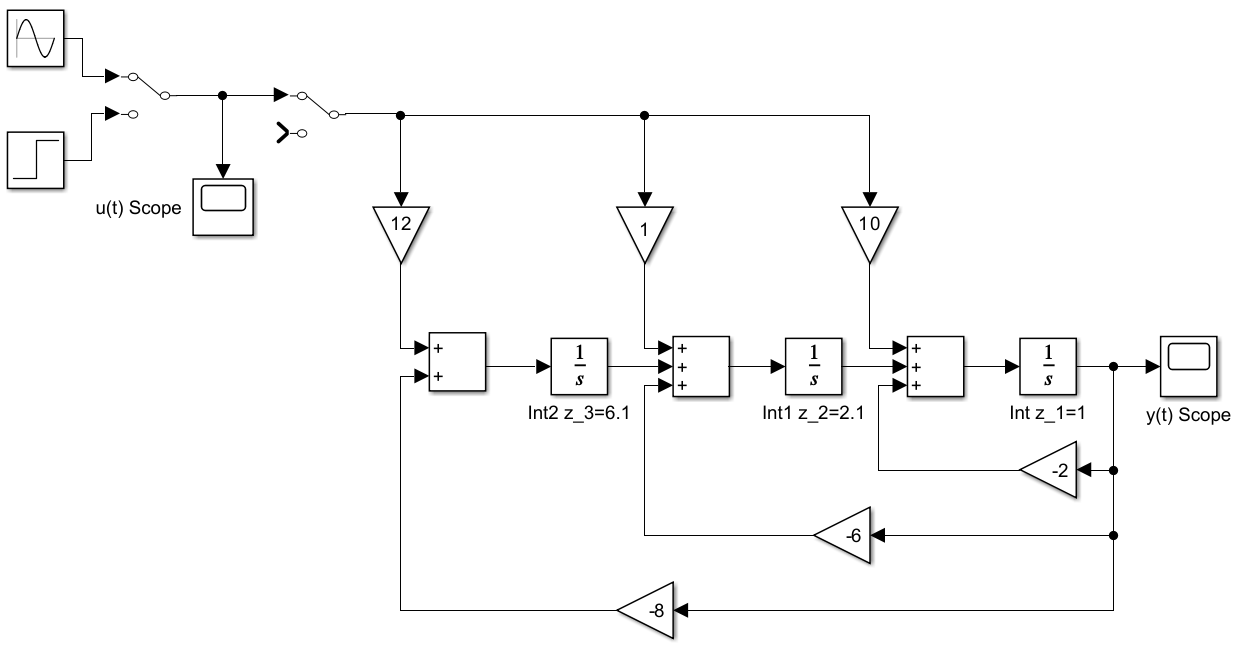
\includegraphics[scale=0.5]{scheme1.png}
        \captionsetup{skip=0pt}
        \caption{Схема моделирования на основе составленного уравнения}
        \label{fig:scheme1}
    \end{figure}
    Зададим нулевое воздействие на систему по условию и выведем результаты $u(t)$ и $y(t)$.
    Продолжительность интервала наблюдения выбрана $[0,30]$.
    \begin{figure}[H]
        \centering
        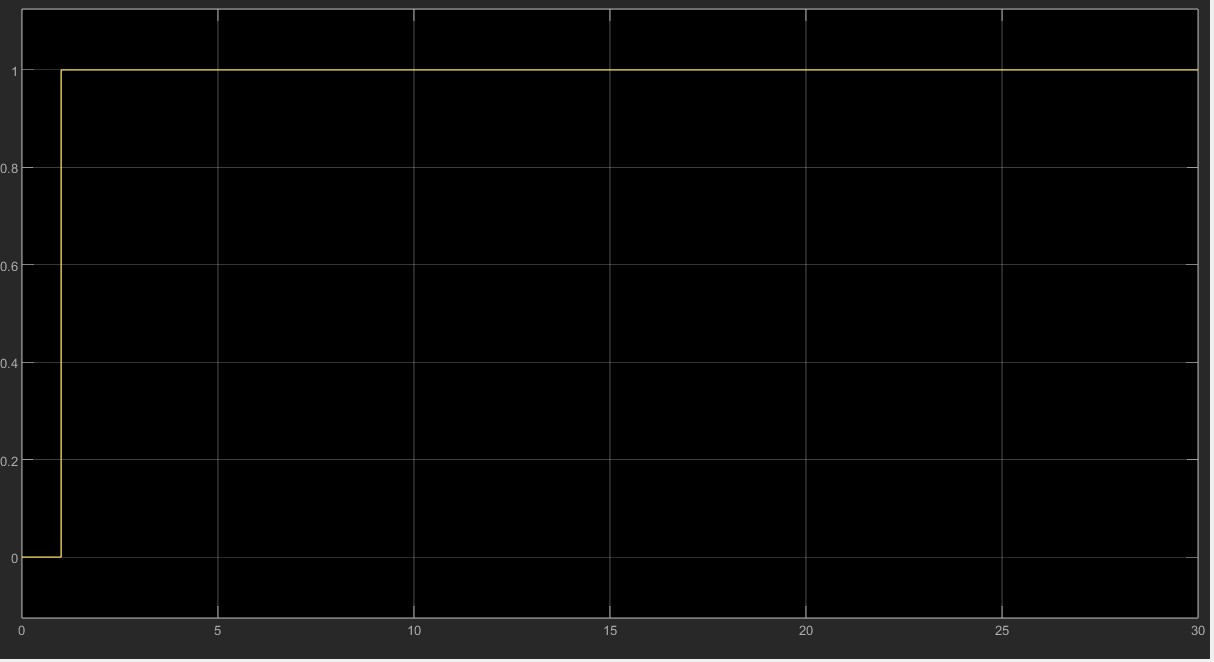
\includegraphics[scale=0.3]{1_t_u.jpg}
        \captionsetup{skip=0pt}
        \caption{Входной сигнал $u(t)$ функции Хевисайда}
        \label{fig:1tu}
    \end{figure}
    \begin{figure}[H]
        \centering
        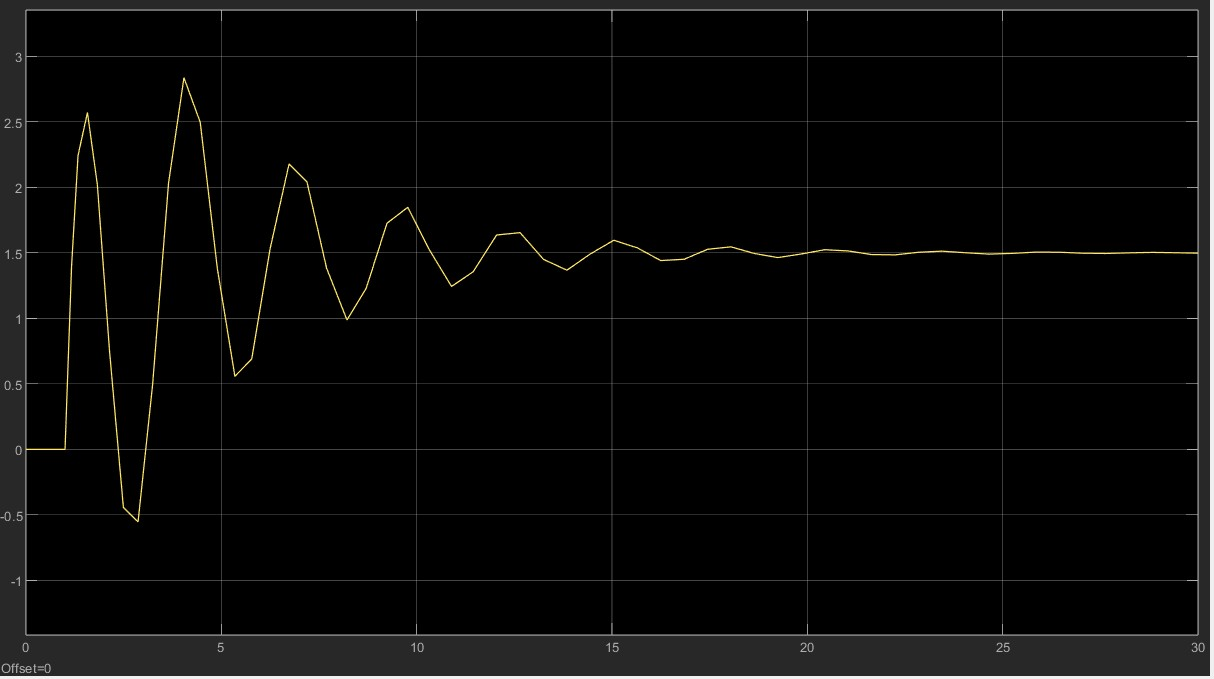
\includegraphics[scale=0.3]{1_t_y.jpg}
        \captionsetup{skip=0pt}
        \caption{Выходной сигнал $y(t)$ функции Хевисайда}
        \label{fig:1ty}
    \end{figure}
    \begin{figure}[H]
        \centering
        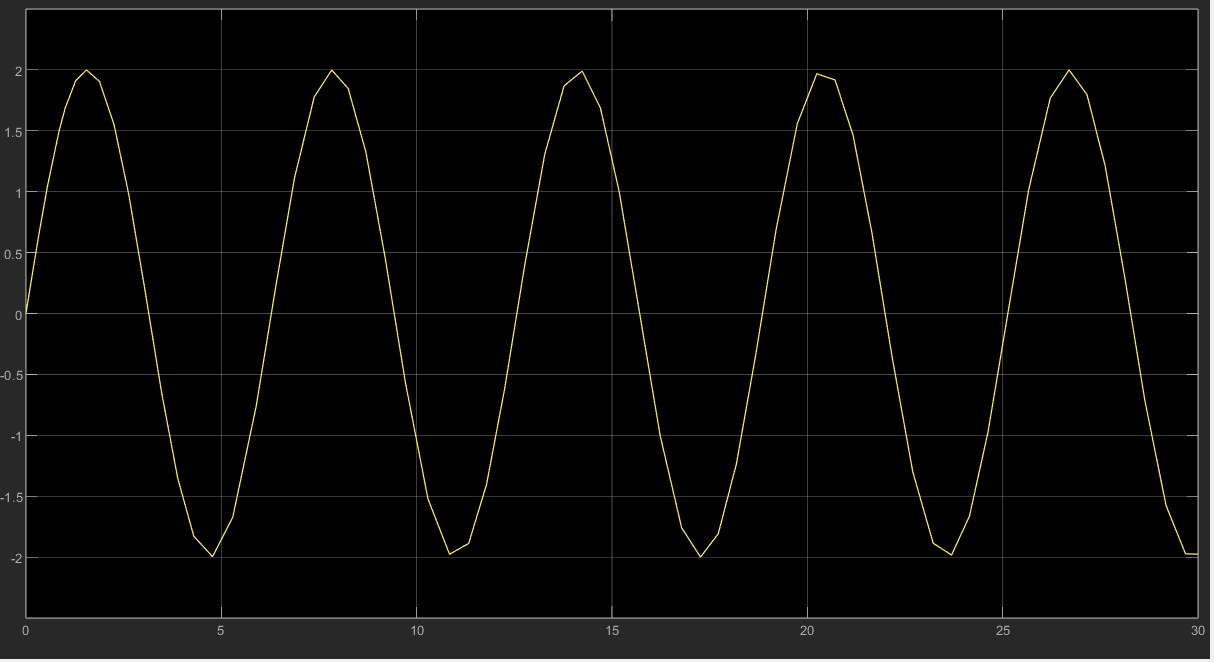
\includegraphics[scale=0.3]{sin_u.jpg}
        \captionsetup{skip=0pt}
        \caption{Входной сигнал $u(t)$ функции синуса}
        \label{fig:sinu}
    \end{figure}
    \begin{figure}[H]
        \centering
        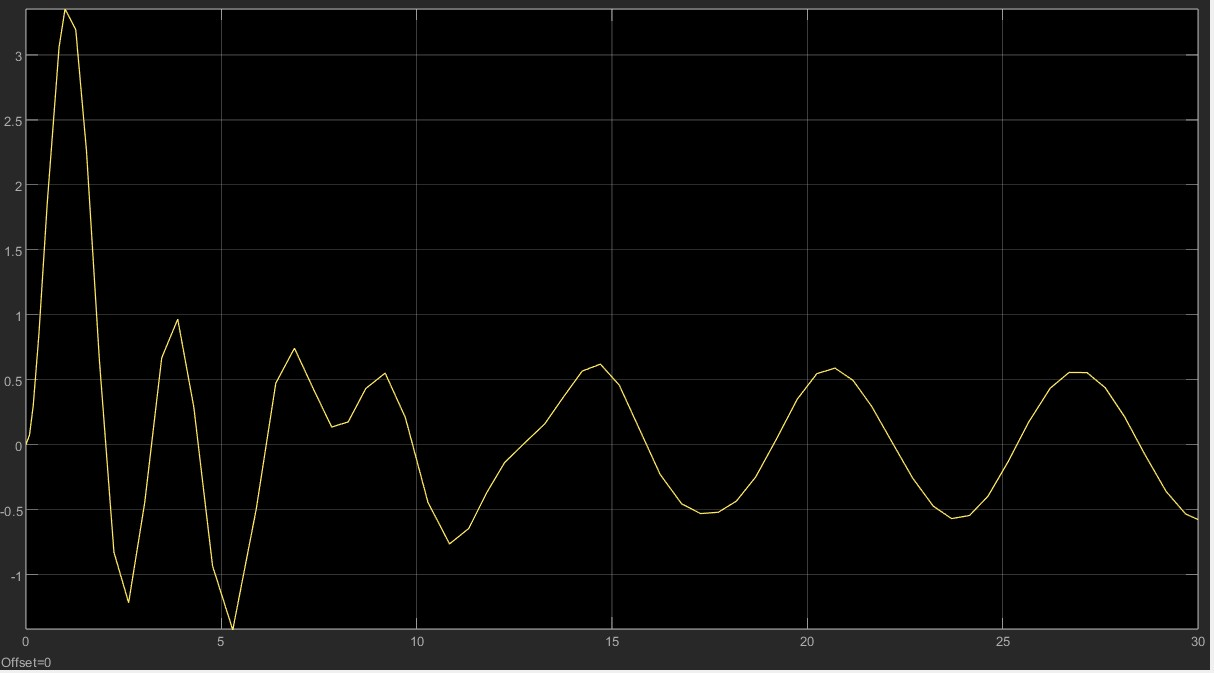
\includegraphics[scale=0.3]{sin_y.jpg}
        \captionsetup{skip=0pt}
        \caption{Выходной сигнал $y(t)$ функции синуса}
        \label{fig:siny}
    \end{figure}

   
    \newpage
    Определим начальные условия интеграторов. Для удобства обозначим выходные сигналы интеграторов
    через $z_1,z_2,z_3$, и, следовательно, искомые начальные условия -- через $z_1(0),z_2(0)$ и $z_3(0)$.
    Так как $z_1=y$, то $z_1(0)=y(0)=1$. Из схемы моделирования \ref{fig:scheme1} видно, что 
    $$\dot{y}=\dot{z}_1=z_2+10u-2y$$
    Выразим $z_2$
    $$z_2=\dot{y}-10u+2y$$
    Подставим начальные значения сигналов $y(0),u(0),\dot{y}(0)$, чтобы вычислить начальное условие для
    второго интегратора
    $$z_2(0)=\dot{y}(0)-10u(0)+2y(0)=0.1-0+2=2.1$$
    Так же из структурной схемы получаем, что
    $$\dot{z}_2=z_3+u-6y$$
    Выразим $z_3$
    $$z_3=\dot{z_2}-u+6y$$
    Продифференцируем $z_2$, которое выразили ранее из $\dot{z}_1$, и, подставим результат в $z_3$
    $$\dot{z}_2=\ddot{y}-10\dot{u}+2\dot{y}\Rightarrow z_3=\ddot{y}-10\dot{u}+2\dot{y}-u+6y$$
    Подставим начальные значения сигналов и вычислим начальное условие для третьего интегратора
    $$z_3=\ddot{y}(0)-10\dot{u}(0)+2\dot{y}(0)-u(0)+6y(0)=-0.1-0+2\cdot0.1-0+6\cdot1=6.1$$
    Напоминание: начальные условия слева $\Rightarrow u(0)=\dot{u}(0)=0$. Выведем результат $y(t)$.
    \begin{figure}[H]
        \centering
        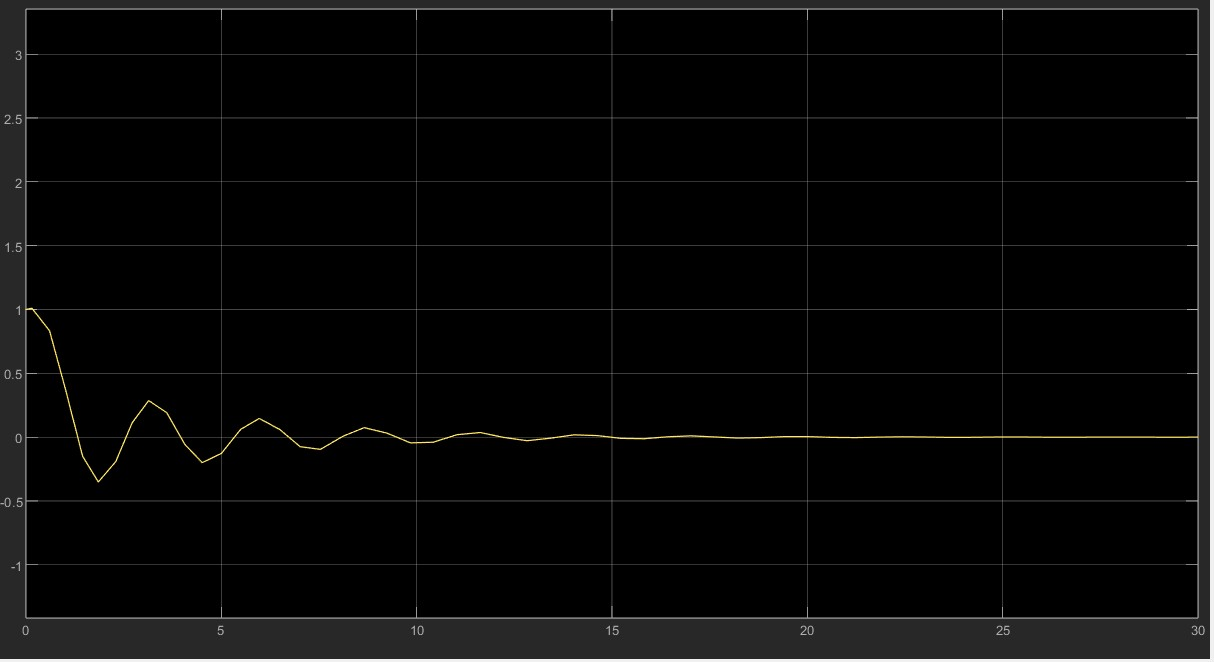
\includegraphics[scale=0.3]{null_y.jpg}
        \captionsetup{skip=0pt}
        \caption{Выходной сигнал $y(t)$ при свободном движении системы}
        \label{fig:null_y}
    \end{figure}


    \section{Задание 2}
    \subsection{Условие}
    \textit{Исследование модели вход-состояние-выход:}
    \begin{compactitem}
    \item Построить схему моделирования линейной динамической системы при
    $$n=2,\ \
    A=
    \begin{bmatrix}
        0 & -4\\
        1 & -1
    \end{bmatrix},\ \
    B=
    \begin{bmatrix}
        0.5\\
        0.25
    \end{bmatrix},\ \
    C^T=
    \begin{bmatrix}
        0\\
        8
    \end{bmatrix}$$
    \item Осуществить моделирование линейной динамической системы при двух видах входного воздействия
    $$u=1(t),\ \ u=2\sin{(t)}$$ Выводить графики
    сигналов $u(t)$ и $y(t)$. Начальное значение вектора состояния нулевое.
    \item Осуществить моделирование свободного движения системы с начальными условиями
    $$x_1(0)=-0.5,\ \ x_2(0)=0.13$$ Выводить графики $y(t)$.
    \end{compactitem}


    \subsection{Выполнение}
    Математическая модель линейной стационарной системы может быть представлена в виде системы
    из $n$ дифференциальных уравнений 1-го порядка (модель \textit{вход-состояние-выход}).
    Запишем ее в компактной векторно-матричной форме
    $$
    \begin{cases}
        \dot{x}=Ax+Bu\\
        y=Cx
    \end{cases}
    $$
    где $A$ -- $n\times n$ матрица постоянных коэффициентов, $B$ -- $n\times1$ вектор-столбец постоянных
    коэффициентов, $C$ -- $1\times n$ вектор-строка постоянных коэффициентов, а $x$ -- $n$-мерный вектор состояния.
    Исходя из данных в задаче, запишем систему, которой будет описываться динамическая система
    $$
    \begin{cases}
    \dot{x}_1=0x_1-4x_2+0.5u\\
    \dot{x}_2=1x_1-1x_2+0.25u\\
    y=0x_1+8x_2
    \end{cases}
    \Rightarrow
    \begin{cases}
        \dot{x}_1=-4x_2+0.5u\\
        \dot{x}_2=x_1-x_2+0.25u\\
        y=8x_2
    \end{cases}
    $$
    Составим схему моделирования системы (рис. \ref{fig:scheme2}).
    \begin{figure}[H]
        \centering
        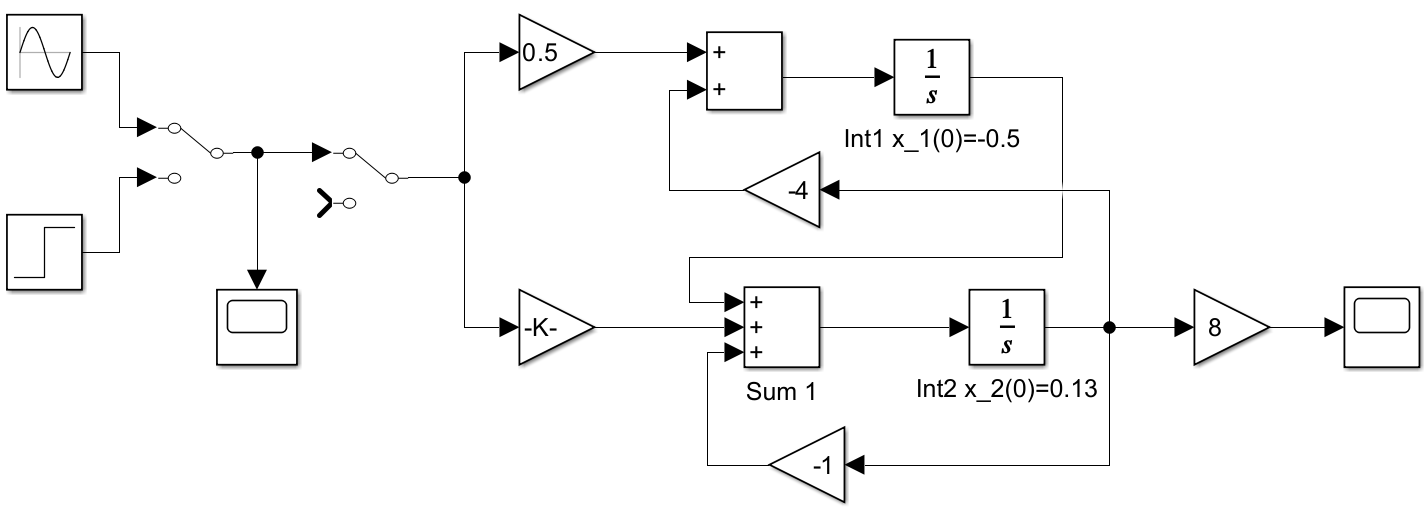
\includegraphics[scale=0.435]{scheme2.png}
        \captionsetup{skip=0pt}
        \caption{Схема моделирования на основе составленной системы}
        \label{fig:scheme2}
    \end{figure}
    Зададим нулевое воздействие на систему по условию и выведем результаты $u(t)$ и $y(t)$.
    Продолжительность интервала наблюдения выбрана $[0,30]$.
    \begin{figure}[H]
        \centering
        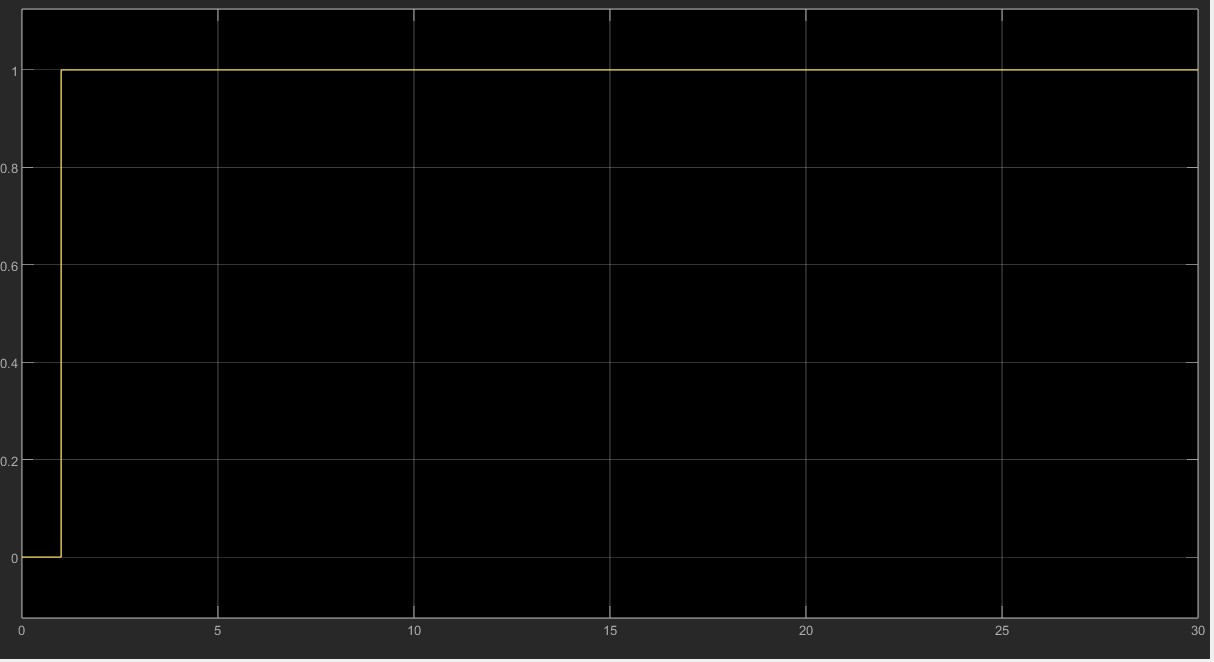
\includegraphics[scale=0.3]{1_t_u_2.jpg}
        \captionsetup{skip=0pt}
        \caption{Входной сигнал $u(t)$ функции Хевисайда}
        \label{fig:1_t_u_2}
    \end{figure}
    \begin{figure}[H]
        \centering
        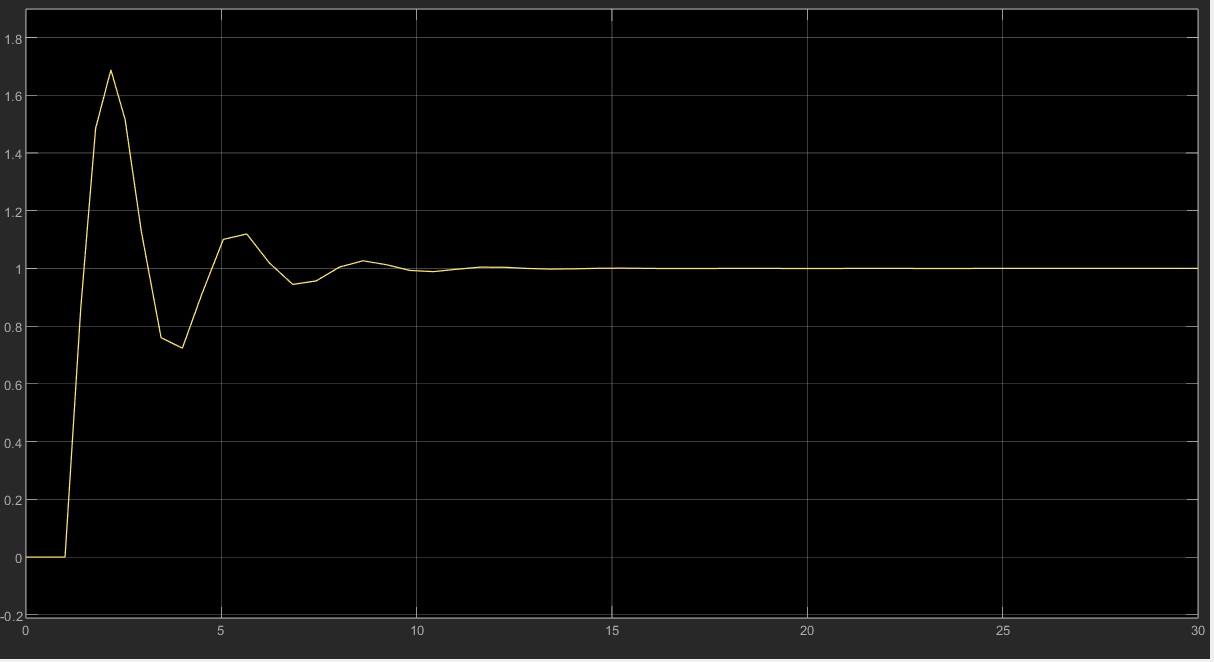
\includegraphics[scale=0.3]{1_t_y_2.jpg}
        \captionsetup{skip=0pt}
        \caption{Выходной сигнал $y(t)$ функции Хевисайда}
        \label{fig:1_t_y_2}
    \end{figure}
    \begin{figure}[H]
        \centering
        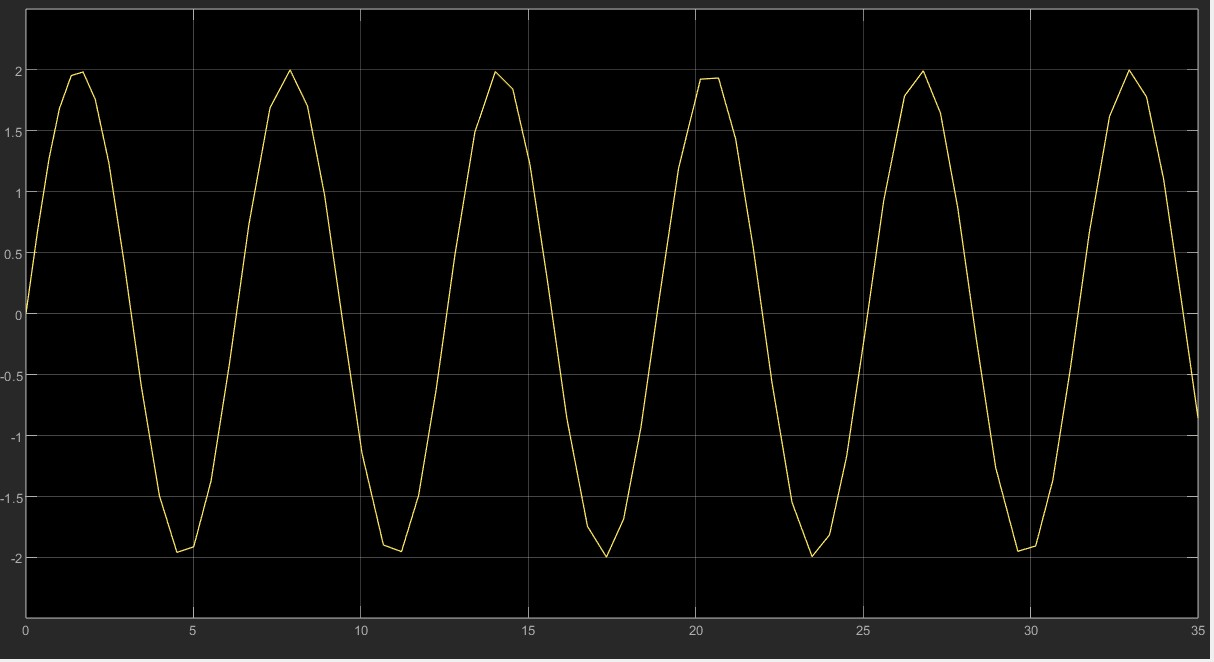
\includegraphics[scale=0.3]{sin_u_2.jpg}
        \captionsetup{skip=0pt}
        \caption{Входной сигнал $u(t)$ функции синуса}
        \label{fig:sin_u_2}
    \end{figure}
    \begin{figure}[H]
        \centering
        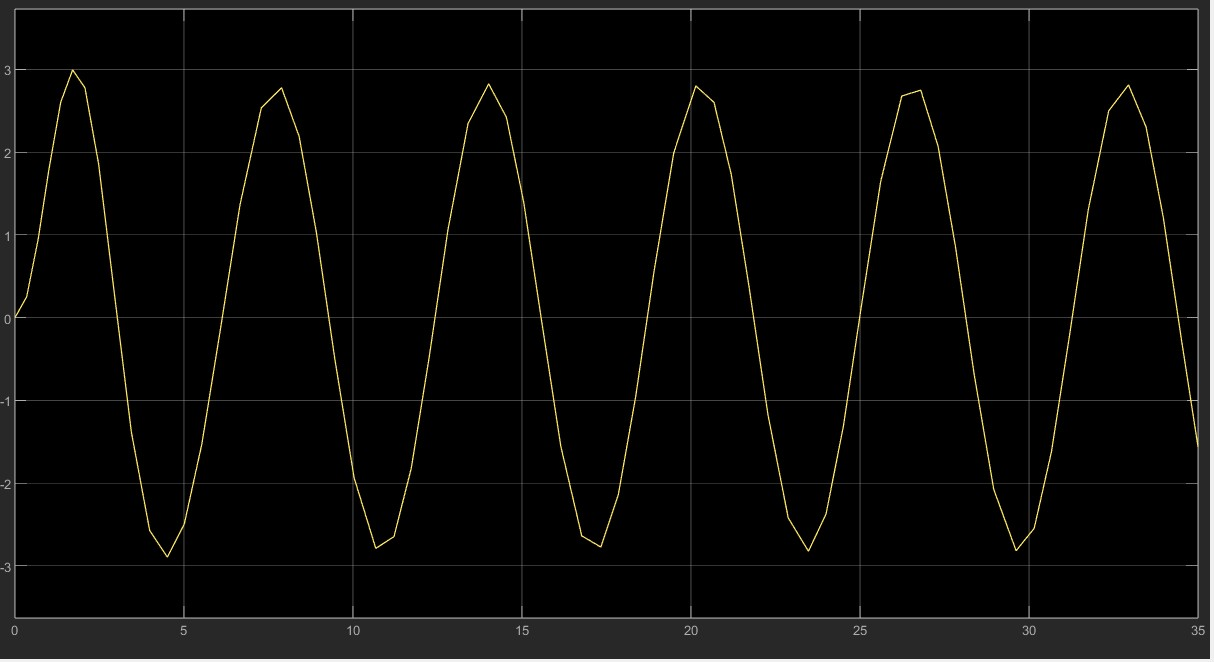
\includegraphics[scale=0.3]{sin_y_2.jpg}
        \captionsetup{skip=0pt}
        \caption{Выходной сигнал $y(t)$ функции синуса}
        \label{fig:sin_y_2}
    \end{figure}
    Начальные условия на интеграторах соответствуют начальным значениям координат вектора состояния $x_1(0)$ и $x_2(0)$.
    Выведем график $y(t)$.
    \begin{figure}[H]
        \centering
        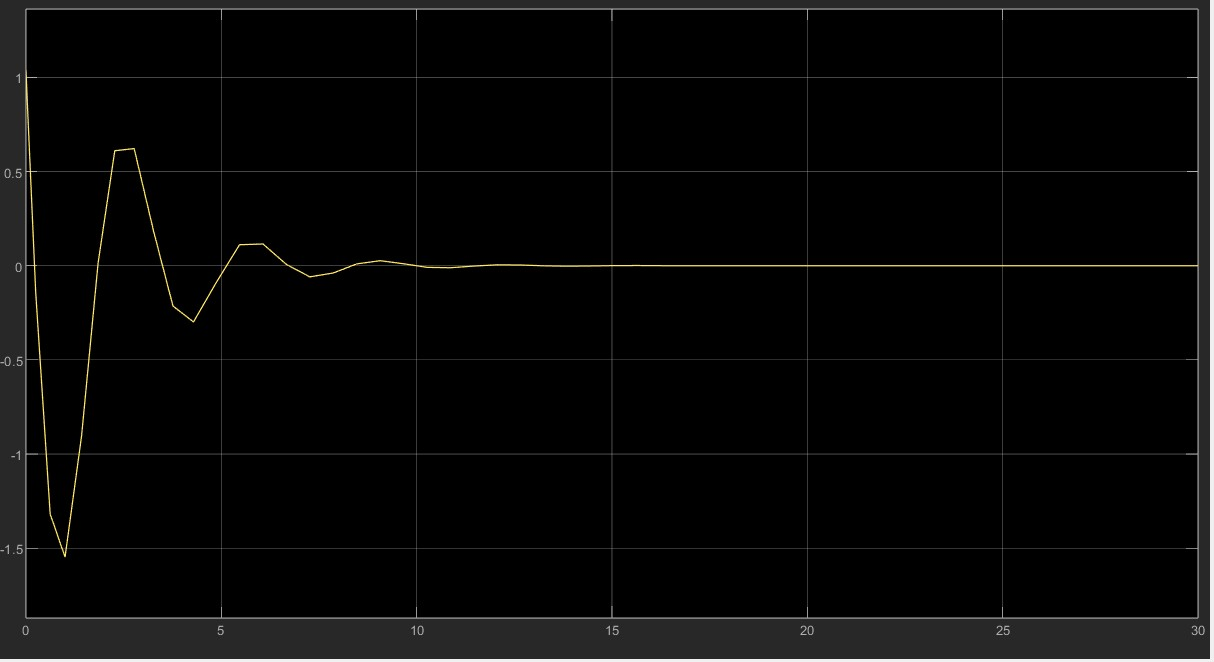
\includegraphics[scale=0.3]{null_y_2.jpg}
        \captionsetup{skip=0pt}
        \caption{Выходной сигнал $y(t)$ при свободном движении системы}
        \label{fig:null_y_2}
    \end{figure}


    \section{Вывод}
    В ходе выполнения данной лабораторной работы я научился пользоваться пакетом
    прикладных программ SIMULINK и познакомился с основными способами моделирования линейных динамических систем.
\end{document}